\section{Was ist maschinelles Lernen?} \label{ch:what_is_ml}

\subsection{Maschinelles Lernen allgemein}

Normalerweise besteht die Aufgabe der Programmierung darin, Regeln auf bestimmte Probleme anzuwenden, um Lösungen zu erhalten.
Mit Hilfe des maschinellen Lernens wollen wir ein Modell erstellen, das Lösungen für bestimmte Probleme verwendet, um die entsprechenden Regeln herauszufinden.
Das Verhältnis wird in Abbildung~\ref{fig:cp_vs_ml} dargestellt.

\begin{figure}
    \centering
    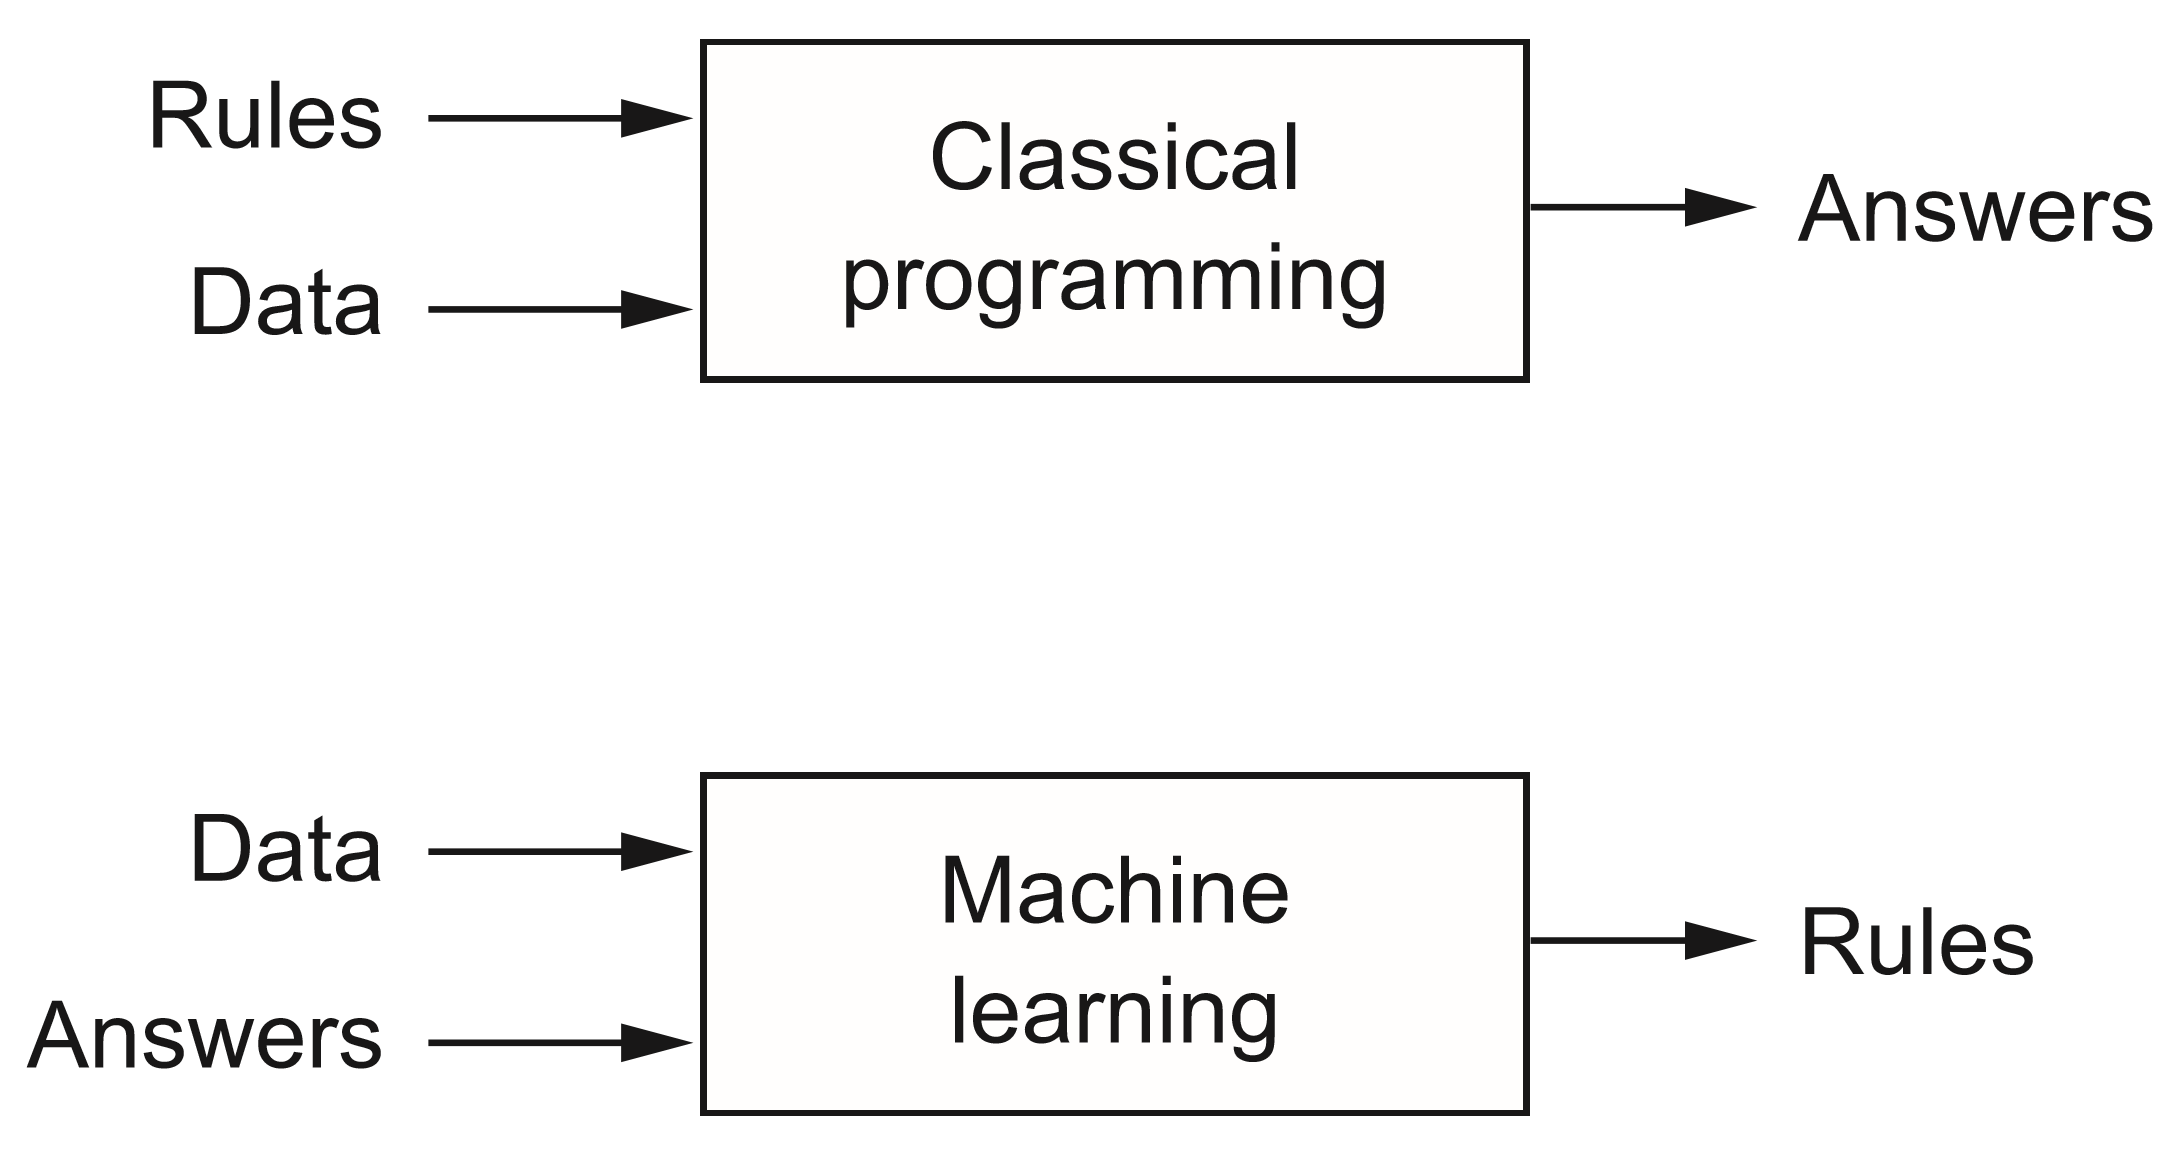
\includegraphics[width=0.5\textwidth]{images/classical_prog_vs_ml.png}
    \caption{Maschinelles Lernen, ein neues Programmierparadigma, von \cite[S.5]{Chollet2017}}
    \label{fig:cp_vs_ml}
\end{figure}

Das Versprechen des maschinellen Lernens ist, dass die gelernten Regeln wesentlich komplexer sein können, als es möglich ist, sie von Hand zu programmieren.
Ein gutes Beispiel dafür ist die Bilderkennung (die im Mittelpunkt dieses Projekts stehen wird), bei der der Inhalt von Bildern klassifiziert werden soll.
Die Beziehungen zwischen den Pixeln müssen herausgefunden werden, was zu einem ziemlich komplexen Modell führt.
Dies ist selbst für die einfachsten Aufgaben nicht auf traditionelle Weise zu programmieren.

Das universelle Approximationstheorem \cite{Cybenko1989} \cite{Hornik1989} besagt, dass es für eine beliebige Eingabe $x$ eine Funktion $h$ gibt, die sich der Zuordnung $y$ annähert, während die Zuordnung nur die Eingabe zur jeweils richtigen Ausgabe (oft von einem Menschen beschriftet) ist.
Diese Beziehung wird in Gleichung~\eqref{eq:universal_approx} gezeigt.

\begin{equation}
    \forall \epsilon > 0 :
    \exists h(\theta, x) : \forall x \in I : | h(\theta, x) - y(x) | < \epsilon
    \label{eq:universal_approx}
\end{equation}

Die mathematische Beschreibung von $h$ wird als Modell bezeichnet (z.B. $h(x) = \sum_{i=1}^n{\lambda (\theta^T * x)}$).
$\lambda \in \mathbb{R}$ ist eine Konstante und $\theta$ ist ein Tensor, der die Parameter von $h$ definiert, die sich aus so genannten Weights und Biases zusammensetzen, die später näher erläutert werden.

Das universelle Approximationstheorem macht keine Aussagen über die Form von $\theta$; daher wird $h$ als Hypothese bezeichnet, weil es besagt, dass für eine bestimmte Zusammensetzung von $\theta$ diese Gleichung zutrifft.
Dieser Begriff wird in der Gleichung~\eqref{eq:hypothesis} zusammengefasst.

\begin{equation}
    \forall \epsilon > 0 : \exists \theta \in X : \forall x \in I : |
    h_\theta(x) - y(x) | < \epsilon
    \label{eq:hypothesis}
\end{equation}

Zur Modellbewertung wird eine Verlustfunktion verwendet; sie vergleicht das Ergebnis der Hypothese mit den bereitgestellten Daten.
Die wohl prominenteste Verlustfunktion ist der \name{Mean Square Error}.
Sie nimmt die Summe der Abweichung von $n$-Beispielen zum Quadrat und dividiert sie durch $2*n$.

\begin{equation}
    L_{mse}(\theta, x) = \frac{1}{2 n} \sum_{i=1}^n (h_\theta(x) - y(x))^2
    \label{eq:mse}
\end{equation}

Die Aufgabe des maschinellen Lernens besteht darin, ein $\theta$ für ein Modell zu bestimmen, das die Gleichungen~\ref{eq:universal_approx} und \ref{eq:hypothesis} bestätigt, was durch iterative Aktualisierung des $\theta$ geschieht. 
Vor dem Training wird $\theta$ zufällig initiiert und dann iterativ angepasst, um $\epsilon$ gegen null konvergieren zu lassen. Dadurch wird der Wert von $L$ minimiert.

Damit der Wert der Verlustfunktion allmählich abnimmt, wird $\theta$ mit Hilfe einer Optimierungsfunktion angepasst.
Dies geschieht meist mit einem Gradientenabstiegsalgorithmus oder einer Variante davon.
Der Gradientenabstieg wird durch Berechnung des Gradienten der Verlustfunktion und Subtraktion von den entsprechenden Parametern durchgeführt, die in  Gleichung~\eqref{eq:gradient_descent} dargestellt sind.

\begin{equation}
    \theta_{i+1} := \theta_i - \eta \nabla_\theta L(\theta, x)
    \label{eq:gradient_descent}
\end{equation}

Dabei ist $\eta$ eine Konstante, die als Lernrate bezeichnet wird und die dazu beiträgt, dass die Verlustfunktion mit Hilfe des Gradientenabstiegsalgorithmus auf 0 konvergiert.
Sie ist einer von vielen Hyperparametern, die nicht automatisch während des Trainings angepasst, sondern vorher bestimmt werden.
Eine optimale Einstellung von Hyperparametern ist eine wichtige Aufgabe, die schwer zu automatisieren ist und daher im Mittelpunkt vieler Forschungsarbeiten steht\footnote{Es gibt Algorithmen zur Anpassung der Lernrate, nämlich \name{AdaGrad} \cite{Duchi2010} und abgeleitete Algorithmen.} und ist das Hauptthema des Kapitels \ref{ch:hyper_parameter_tuning}.
Wenn die Gleichung \eqref{eq:hypothesis} für das jeweilige Modell zutrifft, ist sie anschließend für den gegebenen Input ausreichend geeignet.

Nachfolgend werden diese Konzepte anhand eines einfachen Beispiels vorgestellt.

\subsection{Einfaches lineares Beispiel} \label{ch:simple_linear_example}

Als illustratives Beispiel wird ein Modell erstellt, das Fahrenheit in Celsius übersetzt.
Die ursprüngliche Gleichung ist durch die lineare Funktion $y = mx + b$ als $F = C * 1,8 + 32$ gegeben, mit $F$ als Grad Fahrenheit und $C$ als Grad Celsius.

Ein Modell, das diese Beziehung erlernen soll, ist in der Auflistung~\ref{lst:c_to_f} definiert \footnote{Auch verfügbar unter \url{https://aka.klawr.de/srp\#2}} .

\lstinputlisting[label={lst:c_to_f}, caption={Celsius to Fahrenheit}]{code/c_to_f.js}

Das beschriebene Modell ist durch \code{w} und die Hypothesenfunktion durch \code{h} implementiert.
Da bekannt ist, dass die Beziehung linear ist, stellt das Modell ein eindimensionales Polynom dar, wobei der erste Index dimensionslos ist (und wie bereits erwähnt den Bias emuliert) und der zweite als Input x verwendet wird.
Wir werden später eine Dimension hinzufügen, um das Verhalten bei Polynomen zu demonstrieren, die nicht unmittelbar die Zielfunktion darstellen.

\code{y} liefert die richtige, vorgegebene Lösung.
Bitte beachten Sie, dass \code{y} nur während des Trainings verwendet wird und weggelassen wird, wenn die Modellparameter nach dem Training richtig eingestellt sind.

In diesem Beispiel wird die Verlustfunktion durch den \textit{mean square error } beschrieben \footnote{ abgekürzt als \textit{mse}, welche in Gleichung~\eqref{eq:mse} gezeigt wird.}

Zur Minimierung der in Gleichung~\eqref{eq:gradient_descent} beschriebenen Verlustfunktion wird der Gradientenabstieg verwendet.

In listing~\ref{lst:c_to_f} wird Gleichung~\eqref{eq:gradient_descent} als \code{sgd} mit $\theta_0 = \code{b}$ und $\theta_1= \code{m}$ implementiert, wie in Gleichung~\eqref{eq:sgd_mse_here} gezeigt.

\code{sgd} ist die Abkürzung für \textit{stochastic gradient descent}(zu deutsch: stochastischer Gradientenabstieg)\footnote{Es wird unterschieden zwischen Batch, Mini-Batch und stochastischem Gradientenabstieg; unter Verwendung eines vollständigen Datensatzes, eines definierten Teilsatzes oder einzelner Daten auf die einzelnen Iterationen des Trainingsprozesses.}.
Sie stellt die Optimierungsfunktion dar, die die Parameter des Modells aktualisiert, indem sie den Gradienten des Verlusts für jeden einzelnen Parameter berechnet und sie anschließend aktualisiert.

\begin{equation}
    \begin{split}
        \theta_{0} & := \theta_{0} - \frac{\partial L}{\partial \theta_{0}} =
        \theta_{0} - (h(x) - y(x))  \\
        \theta_{1} & := \theta_{1} - \frac{\partial L}{\partial \theta_{1}} =
        \theta_{0} - (h(x) - y(x)) * x
    \end{split}
    \label{eq:sgd_mse_here}
\end{equation}

Die jeweilige Ausgabe sieht dann in etwa so aus:
\begin{lstlisting}
    loss:  343041.666256673
    loss:  16242.7707476548
    loss:  88.27595280422442
    loss:  10.74432403839251
    loss:  1.1607137779951606
    loss:  0.252186283500194
    loss:  0.00040450626910586374
    loss:  0.00004247033303206121
    loss:  7.158429555712516e-7
    loss:  1.6948019668728757e-10
    weights:  [ 31.99999973758735, 1.8000003977458756 ]
\end{lstlisting}

Das erwartete Verhalten für die Verlustfunktion ist, bei jeder Iteration abzunehmen.
In diesem Beispiel ist dies der Fall und damit wird gezeigt, dass die Abweichung der Hypothese vom tatsächlichen Ergebnis abnimmt.
Nach 200 Iterationen werden die Parameter \code{m} und \code{b} des \code{Modells} ausgegeben und zeigen, dass sie tatsächlich nahe am erwarteten Ergebnis liegen.
Durch Erhöhen der Iterationszahl kann das Ergebnis bis zu dem Punkt erhöht werden, an dem sie vom JavaScript-Compiler gerundet werden, um exakte Ergebnisse darzustellen (unter Verwendung von Node.js\footnote{ Soweit bei der Berechnung exakter Ergebnisse unter Verwendung von Fließkommazahlen eben angenommen werden können.}).

\begin{SCfigure}
    \centering
    \caption{Das vorliegende Beispiel kann wie hier dargestellt visualisiert werden. Der Bias kann als zusätzlicher Input interpretiert werden, welcher stets den Wert 1 hat. Die Eingabe wird mit den Parametern multipliziert, die mit den entsprechenden Pfeilen gekennzeichnet sind, die wiederum aufsummiert werden (daraus resultiert $y = mx + b$).}
    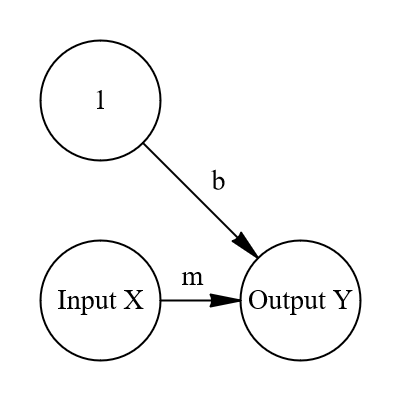
\includegraphics[width=0.5\textwidth]{images/1_simplest_nn.png}
\end{SCfigure}

Vorausgesetzt, dass diese Hypothese anfangs gut für die Aufgabe geeignet ist, ist es wichtig zu beachten, dass durch die Modifizierung der Hypothese zur Darstellung eines Polynoms höheren Grades (z.B. $y = nx^2 + mx + b$) die zusätzlichen Parameter gegen 0 konvergieren, was effektiv das gleiche Ergebnis wie zuvor liefert \footnote{Aber um ähnliche Ergebnisse zu erzielen, muss die Iterationszahl mindestens um den Faktor 20 erhöht werden.
Das Experiment kann unter \url{https://aka.klawr.de/srp\#3}} nachvollzogen werden.
